\subsection{Trees}

\subsubsection{Definitions and characteristics}

Before introducing what a tree is, it is necessary to understand what a subgraph is. Mathematically speaking, $G'= \left(N', E'\right)$ is a \definitionWithSpecificIndex{subgraph}{Subgraph} of $G = \left(N,E\right)$ if $N' \subseteq N$ and $E' \subseteq E$.

\highspace
A \definitionWithSpecificIndex{tree of the graph $G$}{Tree of a graph} is a connected and acyclic subgraph of $G$ and it is represented as $G_{T} = \left(N', T\right)$. If the tree contains exactly every node in the graph $G$, it is called the \definitionWithSpecificIndex{spanning tree}{Spanning tree} of $G$ and is represented as $G_{T} = \left(N', T\right)$. Finally, we call the \textbf{nodes of degree 1} in a tree as \definitionWithSpecificIndex{leaves}{Leaves of a tree}.

\begin{examplebox}[: subgraph, tree and spanning tree]
    Given a graph $G$:
    \begin{center}
        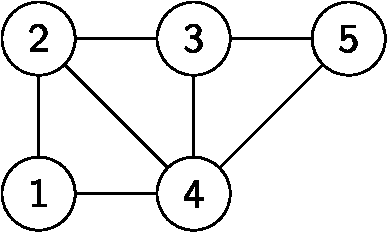
\includegraphics[width=.3\textwidth]{img/trees-1.pdf}
    \end{center}

    \begin{itemize}
        \item The following figure is a \textbf{subgraph} of $G$, but \underline{not} a tree, because there is a cycle $\left(1,2,4\right)$.
        \begin{center}
            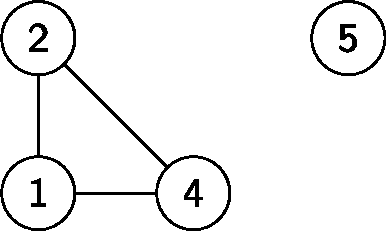
\includegraphics[width=.3\textwidth]{img/trees-2.pdf}
        \end{center}

        \item The following figure is a \textbf{subgraph} of $G$, and it is a \textbf{tree} because there are no cycles and the graph is connected.
        \begin{center}
            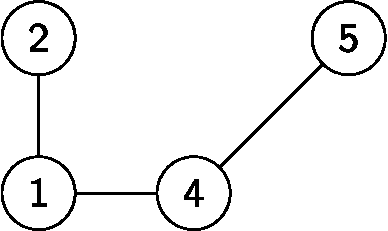
\includegraphics[width=.3\textwidth]{img/trees-3.pdf}
        \end{center}
        
        \item The following figure is a \textbf{spanning tree} of $G$ because it contains all the nodes in $G$, and it is a tree because it is connected and acyclic.
        \begin{center}
            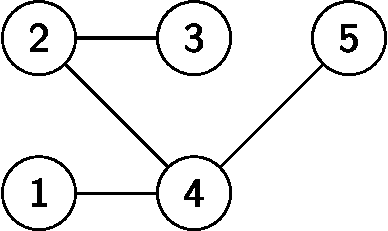
\includegraphics[width=.3\textwidth]{img/trees-4.pdf}
        \end{center}
    \end{itemize}
\end{examplebox}